\chapter{Theory}
\label{cha:theory}

Theories used in this study are presented here. They include software
development methodology, software metrics, reactive systems and some general
information regarding the \textit{libuv} library.

\section{Internet of Things}

\todo{A bit messy intro, perhaps mention different viewpoints of IoT and try to
find common demoninators among them.}

The Internet of Things (IoT) is a relatively new paradigm of the internet where
not only people are interconnected, but \textit{everything} is. The term was
first heard in 1999 in a presentation by Kevin Ashton \cite{ashton2011internet}
and the popularity has since blossomed \cite{gubbi2013internet}. IoT can be
conceptualized as context-aware \textit{things} communicating with each other
and human-centered applications. The enabling applications are vast and include
domains from many areas of society - transportation, healthcare, homes, offices
and social domains to name a few. A good example is electricity consumption
control in homes. Electricity prices can be monitored and utilities such as
washing machines and heating can be optimized and only used when prices are low
\cite{atzori2010internet}. IoT can typically be explained as "one paradigm with
many visions" \cite{atzori2010internet} as there is no official definition of
the term. IoT is more than ubiquitous computing, embedded devices and
applications. It should not only be accessible by a small group of stakeholders
but embedded in today's open internet infrastructure. Referring to logistics an
IoT definition can be viewed as \textit{"[asking] for the right product in the
right quantity at the right time at the right place in the right condition and
at the right price"} \cite{uckelmann2011architectural}. Uckelmann et. al.
discusses these approaches and defines IoT as:

\begin{center}
\textit{"Internet of Things links
uniquely identifiable things to their virtual representations in the Internet
containing or linking to additional information on their identity, status,
location or any other business, social or privately relevant information at a
financial or non-financial pay-off that exceeds the efforts of information
provisioning and offers information access to non-predefined participants. The
provided accurate and appropriate information may be accessed in the right
quantity and condition, at the right time and place at the right price. The
Internet of Things is not synonymous with ubiquitous / pervasive computing, the
Internet Protocol (IP), communication technology, embedded devices, its
applications, the Internet of People or the Intranet / Extranet of Things, yet
it combines aspects and technologies of all of these approaches."}
\cite{uckelmann2011architectural}.
\end{center}

\subsection{Enabling technologies and challenges}

The state-of-the-art technologies used today in the IoT context include
sensoring equipment and networks such as the \textit{Radio Frequency
Identification} (RFID) and the \textit{Wireless Sensor Network} (WSN),
communication techniques like the \textit{IPv6 over Low-Power Wireless Personal
Area Network} (6LoWPAN) and \textit{Representational State Transfer} (REST) and
architectural approaches like \textit{middleware} and \textit{gateways}.

The RFID is a technique used to identify an object by letting a reader generate
an electromagnetic wave which in turn generates a current in a microchip that
transmits a code back to the reader. The code, also known as an
\textit{Electronic Product Code} (EPC), can be used to identify the object. EPC
is developed by EPCglobal, a global non-profit organization, with the purpose
to spread the use of RFID and create global standards for modern businesses
\cite{atzori2010internet}. An RFID tag can be passive, i.e. work without
battery power, or active, i.e. work with battery power. It basically consists
of an antenna, a microchip attached to the antenna and some form of
encapsulation. They vary in size and shape; from centimeter long 3D-shaped
capsules to 2D-shaped stickers. The fact that they can work without a battery,
meaning they theoretically can work forever, make them very practical to use in
different environments. \cite{want2006introduction}

In a survey from 2001, Akyildiz et. al.  \cite{akyildiz2002wireless} presents a
\textit{Wireless Sensor Network} containing hardware nodes capable of
monitoring its environment and transmit the received data to a server or host
acting as a sink. The sensor could be one of many types and be able to measure
temperature, humidity, movement, lightning condition, noise levels etc. This
leads into one of the major challenges in IoT: communication and networking.
Following the semantical meaning of IoT, which states \textit{"[it is] a world
wide network of interconnected objects uniquely addressable, based on standard
communication protocols"} \cite{bassi2008internet}, it is clear that every node
will produce its own content and should be retrievable regardless of location.
This puts pressure on the identification methods and the overall network
infrastructure for IoT. As remaining unused IPv4 addresses are closing in to
zero, the IPv6 protocol can be a natural next step for IoT devices to use
\cite{atzori2010internet}. 4 bytes are used to address devices in IPv4, wich
means the protocol can support around 4 billion devices. IPv6 on the other hand
use 16 bytes to address devices, meaning around $10^{38}$ devices can be
uniquely addressed.

6LoWPAN is a wireless technology suitable for resource-constrained nodes in the
IoT network. It is designed for small packet sizes, low bandwidth, low power
and low cost. It assumes a large amount of nodes will be deployed and that they
can be unreliable in terms of radio connectivity and power drain, thus making
this technology a good choice for wireless sensor nodes. \cite{kushalnagar2007ipv6}

\todo{REST?}

\subsection{Gateways}

A big challenge in IoT is, as described earlier, to connect every single device
to the internet. As for example devices in a WSN are deployed they do not
necessarily have the power and capacity to directly communicate to the
internet. A common approach to solve this problem is to add a gateway between
the devices and the internet, acting as an amplifier for the transmissions from
the devices \cite{zhu2010iot}. Chen et. al. \cite{chen2011brief} describes three
layers of domains in the IoT architecture: the \textit{sensing domain}, the
\textit{network domain} and the \textit{application domain}. The sensing domain
is where the primitive communication between the actual devices in the network
happen; for instance RFID and 6LoWPAN. This domain is layered under the network
domain and each piece of information sent from the sensing domain is
aggregated, filtered and wrapped in the network domain before being sent to the
application domain. Note that the information protocols used between the
sensing- and network domain and the network- and application domain does not
necessarily match. As some protocols are more suited for resource-constrained
devices, they might require modification to be able to communicate with more
standardized protocols, like the \textit{Internet Protocol} (IP). E.g. the EPC
code generated by the RFID can not be put on an IP stack as is, but it could be
mapped to an IPv6 address via a gateway and thereby be identified and usable
through the internet \cite{lee2007epc}.

The gateways reside in the network domain. They act as a bridge between the
devices and the internet. The approaches towards implementing IoT gateways vary

\todo{Should list different approaches in the industry, from large companies to
smaller projects.}

\section{Event-driven architectures}

In software architecture, the term \textit{event-driven}, or \textit{implicit
invocation}, is used to express the mechanism of function invocation based on
events \cite{garlan1993introduction}. In contrast, \textit{explicit invocation}
refers to a traditional function invocation by function name, e.g.
\lstinline{foo()}. However, a function can be mapped to an event
so that when the event occur, the function is invoked implicitly. Hence the
name implicit invocation. The announcers of events do not know what functions
are registered to the event and cannot make assumptions on event ordering or
how data will be transformed due to the event. This is one disadvantage of this
architecture \cite{garlan1993introduction}. However, in high-performance, I/O
intensive networking systems, it is shown that event-based approaches perform
much better \cite{hu1997measuring}.

%% Also, there are research showing that event-driven systems are slower for
%% CPU intense applications.

\subsection{Task management and stack management}

A program task is an encapsulation of control flow with access to some common
shared state. This can be viewed as a closure in a program language or a
function. Managing these tasks can be done in several ways. In
\textit{preemptive} task management, tasks can be scheduled to interleave and
make room for other tasks or be run in parallell on multicore systems. In
\textit{serial} task management, tasks are run until they are finished before
any other task can start its execution. A hybrid approach is
\textit{cooperative} task management. Tasks can yield control to other tasks in
defined points in its execution. This is useful in I/O intensive systems where
tasks can make way for other tasks while waiting for I/O. Event-driven systems
usually implements the cooperative approach. Events, e.g.  network requests,
are handled by calling an associated function. A benefit with event-driven
systems that run on a single thread is that mutual exclusion conflicts never
occur. However, the state in which the task was in before yielding control to
another task is not necessarily the same as when the task resumes control.
\cite{adya2002cooperative}

There are two categories of I/O management: \textit{synchronous} and
\textit{asynchronous} \cite{adya2002cooperative}. If a function calls an I/O
operation and then blocks the rest of the execution while waiting for the I/O
operation to finish, the function is synchronous. Here is an example of a
synchronous read file-function from the Node.js documentation
\cite{nodejs-docs}:

\lstinputlisting[
  language=javascript,
  caption={Synchronous I/O example in Node.js.},
  label={listing:read_file_sync}
]{figures/read_file_sync.js}

The \lstinline{readFileSync()} function blocks the rest of the execution while
the file is being read, i.e. the file content will be printed before
\textit{"end of code"}. In asynchronous I/O, the function calling the I/O
operation returns immediately but is provided a function to be run when the I/O
is ready. Here is an equivalent implementation but with an asynchronous
function:

\lstinputlisting[
  language=javascript,
  caption={Asynchronous I/O example in Node.js.},
  label={listing:read_file_async}
]{figures/read_file_async.js}

\lstinline{readFile()} does not in this case return anything, but instead let
the event handling system invoke the callback function when the I/O is ready.
The execution continues directly, so \textit{"end of code"} will be printed
before the file content.

An interesting notice to Listing \ref{listing:read_file_async} is that, say a
global state is introduced and is dependent upon by the callback function,
there is no guarantee the state remains unchanged between the
\lstinline{readFile()}- and the \lstinline{callback()}-invocation. This is
similar to the mutual exclusion problem in preemeptive task management where
multiple agents wants to access the same resource concurrently, and problems
like read/write conflicts can occur. But since cooperative task management not
necessarily infer multithreaded environments, concurrent problems can be
avoided. There are however other problems related to understanding and
scalability of the code. In Listing \ref{listing:read_file_sync} one can
observe that all operations happen in the same scope. This is called
\textit{automatic stack management} and it means the task is written as a
single procedure with synchronous I/O \cite{adya2002cooperative}. The current
state of the program is always kept in the local stack and there is no
possibility it can be mutated by other parties. In \textit{manual stack
management} the task is ripped into callbacks, or \textit{event handlers},
which are registered to the event handling system. This can have a negative
impact on the control flow and the global state of the program as tasks are
being broken into functions with separate scopes.

%% compare lambdas to function pointers?

\section{Reactive systems}

Systems required to continually respond to its environment are called
\textit{reactive} systems. Harel and Pnueli \cite{harel1985development}
elaborates on different system dichotomies, for instance deterministic and
nondeterministic systems. Deterministic systems have unique actions which
always generates the same output. Nondeterministic systems do not have that
property and it can cause them to be more difficult to handle. Another
dichotomy is sequential and concurrent systems. Concurrent systems cause
problems which are easily avoidable in sequential ones. For instance the mutual
exclusion problem where it is not always trivial what process owns what
resource and whether it is safe to modify a resource that can be used by
another process. A more fundamental dichotomy is presented by Harel and Pnueli:
\textit{transformational} and \textit{reactive} systems. A transformational
system transforms its input and creates new output. It can continually prompt
for new input. A reactive system is prompted the other way around: from the
outside. It does not necessarily compute any input, but it maintains a
relationship with its outside environment. A reactive system can be
deterministic or nondeterministic, sequential or concurrent, thus making the
transformational/reactive system dichotomy a fundamental system paradigm.
\cite{harel1985development}

\subsection{Specifications for reactive systems}

Harel and Pnueli \cite{harel1985development} presents a method for decomposing
complex system using \textit{statecharts}. Drawn from the theories of
\textit{finite state automata}, a system can be expressed using states. This is
particularily useful for reactive systems that can react to a large amount of
different inputs. One powerful feature with statecharts is its ability to
handle hierarchical states. If a system has a numerous amount of input
combinations, a large set of states must be created which in the long run is
not appropiate in terms of scalability. One solution to this is hierarchical
states in which a state can hold a number of other states. Fundamentally, a
state undergo a transition to another state when an action is performed on that
state. \cite{harel1985development}

Ardis et al \cite{ardis1996framework} created a specification for a telephone
switching system which later was tested on a number of languages. They started
by describing some general properties of the system in a list. In general, the
list had the format:

\begin{enumerate}
\item
  When event $X_1$ occurs,
\begin{enumerate}
\item
  If some condition or property of the system holds true, call action $Y_1$
\item
  Otherwise, call action $Z_1$
\end{enumerate}

\item
  When event $X_2$ occurs,
\begin{enumerate}
\item
  Call action $Y_2$
\end{enumerate}

\item
  And so on...
\end{enumerate}

They then implemented a system fullfilling the requirements in a set of
different languages. Most languages fit well for reactive systems since their
semantic allows and makes it easy to build and define different state machines.
They also did one implementation in C in which they had two solutions: one
using arrays to hold all the different actions and states and one using
switch-blocks.

However, specification of primitive components can still be a challenge.
Non-trivial steps might be required to transition from one state to another.
Hummel and Thyssen \cite{hummel2009behavioral} presents a formal method to
specify a reactive system using stream based I/O-tables. In addition to
generating a simple and understandable description of the system, the method
helps formalize inconsistent requirements.

\section{Reactive programming}

Reactive programming has been proposed to be the solution to implement
event-driven architectures \cite{bainomugisha2013survey}. It is derived from
the \textit{Synchronous Data Flow} (SDF) paradigm \cite{lee1987synchronous}.
SDF is a data flow abstraction used to describe parallell computation.
Functions are presented as nodes in a directed graph and the arcs represent
data paths. Nodes can execute its computation whenever data is available on its
incoming arcs, and nodes with no incoming arcs can execute at any time. This
leads to concurrency since multiple nodes can execute in the same time. One
constraint on this system is that of \textit{side-effects}, which are not
allowed. Nodes cannot mutade any resource accessible by another node unless
they are explicitly connected by an arc.

In the reactive programming paradigm, the notion of time is abstracted away. In
the same way memory can be abstracted away by garbage collection in languages
like Java, the programmer does not have to instruct the program \textit{when}
things will execute, but rather \textit{how} \cite{bainomugisha2013survey}.
Data dependencies and change propagation can be handled automatically by the
language. Consider a simple example:

\begin{lstlisting}[language=C]
int i = 1;
int j = 1;
int k = i + j;
\end{lstlisting}

In a language like C, $k$ will be computed to the value $2$. If $i$ later on is
redefined to another value, say $3$, $k$ will still hold the same value $2$. In
a reactive setting, $k$ will be updated with the latest value of either $i$ or
$j$, even if they change later on in time. It can be viewed such that $k$ is
\textit{dependent} on $i$ and $j$. \cite{bainomugisha2013survey}

Reactive programming has two distinguishing features: \textit{behaviors} and
\textit{events}. Behaviors refer to time-varying vales, e.g. time itself.
Events on the other hand, happen in discrete points in time and describes what
happened. This could be a file that is ready to be written to, a network
request that is available or a keyboard button that was pressed.
\cite{bainomugisha2013survey}

\subsection{A taxonomy}

Bainomugisha et. al. \cite{bainomugisha2013survey} presents a taxonomy with six
fundamental properties considered important features in reactive languages.

\subsubsection{Basic abstractions}

Imperative languages holds basic abstractions in the form of primitives such as
primitive operators and values. Reactive languages holds basic abstractions
such as behaviors and events.

\subsubsection{Evaluation model}

When an event occur, the evaluation model of a reactive language determines how
change is propagated throughout the data dependencies. Propagatation can either
be \textit{push-based}, meaning that data is pushed to its dependencies as soon
as an event occur, or \textit{pull-based}, meaning that computation nodes pull
data when needed. The former is a \textit{data driven} model and is often implemented
using callbacks. A challenge is to find out what nodes does not need to be
recomputed. The pull-based model is said to be \textit{demand driven} as data
is propagated upon request. A disadvantage with this model is that delays
between events and reactions can be long.

\subsubsection{Glitch avoidance}

A \textit{glitch} is when inconsistencies in the data occur due to the way
updates are propagated among the dependencies. Consider the following example:

\begin{lstlisting}[language=C]
int i = j;
int k = i + j;
\end{lstlisting}

$k$ is dependent on $i$ and $j$ and $i$ is on another level dependent on
$j$. If $j$ is updated, the case can be that $k$ is updated before $i$, thus
leading to an inconsistency between $k$ and $i$. Here is an example:


\begin{lstlisting}[language=C]
// j == 1
int i = j;      // i == 1
int k = i + j;  // k == 2

// j == 2, k updated before i
int i = j;      // i == 1
int k = i + j;  // k == 3, should be 4
\end{lstlisting}

These kinds of inconsistencies, or glitches, should be avoided by the language.

\subsubsection{Lifting operators}

\textit{Lifting} in reactive programming refers to the act of making previously
uncompliant operators or functions work with behaviors. Lifting transforms the
type signature of the function and registers the topology of its dependencies
in the dataflow graph. A function $f$ with a non-behavior type $T$ can be
lifted as:

\begin{lstlisting}
f(T) -> flift(Behavior<T>)
\end{lstlisting}

Where $Behavior$ is a behavior-type holding a type $T$. In Flapjax, an reactive
language built upon Javascript, lifting is performed on multiple places to
support behaviors \cite{meyerovich2009flapjax}. Here is an example from the
language:

\begin{lstlisting}[language=javascript]
let time = timerB(1000);
\end{lstlisting}

This looks like traditional, imperative Javascript. However, $timerB$ with the
argument $1000$ starts a timer that yields every second and $time$ will always
be kept up to date with the yielded value. Flapjax performs lifting on, among
others, the addition ($+$) operator:


\begin{lstlisting}[language=javascript]
let time = timerB(1000) + 1;
\end{lstlisting}

The compiler transforms the expression using the $liftB$ function, looking
somewhat like this:

\begin{lstlisting}[language=javascript]
liftB(function(t) { return t + 1 }, timerB(1000));
\end{lstlisting}

This is called \textit{implicit lifting}, meaning that the programmer does not
have to worry about whether the add operator was used on a behavior or not
\cite{bainomugisha2013survey}.

\subsubsection{Multidirectionality}

A property of reactive languages is to support data propagation both from
derived data, as well as the data it is derived from. Consider a distance
converting function:

\begin{lstlisting}[language=C]
double miles = km * 1.61;
\end{lstlisting}

Whenever an updated value on either $miles$ or $km$ is available, the other one
is recalculated as well.

\subsubsection{Support for distribution}

As interactive applications such that web applications are becoming more
popular (whose nature is distributed) it is important for reactive languages to
also support distributed mechanisms.

\section{Choosing programming language for embedded systems}

In embedded systems programming, both hardware and software is important. Nahas
and Maaita \cite{nahas2012choosing} mentiones a few factors to be considered
when choosing a programming language for an embedded system:

\begin{itemize}
\item
  The language must take the resource constraints of an embedded processor
  into account
\item
  It must allow low-level access to the hardware
\item
  It must be able to re-use code components in the form of libraries from other
    projects
\item
  It must be a widely used language with good access to documentation and other
    skilled programmers
\end{itemize}

There is no scientific method for selecting an appropiate language for a
specific project. Selection mostly relies on experience and subjective
assessment from developers. It was however shown in 2006 that over 50 \% of
embedded system projects were developed in C and 30 \% were developed in C++.
Barr \cite{barr1999programming} states that the key advantage of C is that it
allows the developer to access hardware without loosing the benefits of
high-level programming. Compared to C, C++ offer a better object-oriented
programming style but can on the other hand be less efficient.
\cite{nahas2012choosing}

\section{libuv}

libuv is an asynchronous I/O cross-platform library written in C. It is one of
the major core systems of Node.js, a popular JavaScript runtime engine. libuv's
central part is the single-threaded event loop which contains all I/O
operations. The event loop notifies any I/O events in a callback fashion using
abstractions called \textit{handles} and \textit{requests}. Handles are
long-lived structures and are operated on using requests. Requests usually only
represent one I/O operation on a handle. Each I/O operation performed on the
event loop is \textit{non-blocking}, meaning they instantly return and
abstracts away any concurrency necessary. To handle network I/O libuv make use
of platform specific functionality, such as \textit{epoll} for Linux. For file
I/O libuv utilizes its \textit{thread pool} to make the operation non-blocking.
All loops can queue work in this thread pool making it ideal for external
services or systems that do not want to block any I/O. libuv include handles
for \textit{UDP} and \textit{TCP} sockets, file and file system, \textit{TTY},
timers and \textit{child processes}. \cite{libuv-docs}

\begin{figure}[h]
  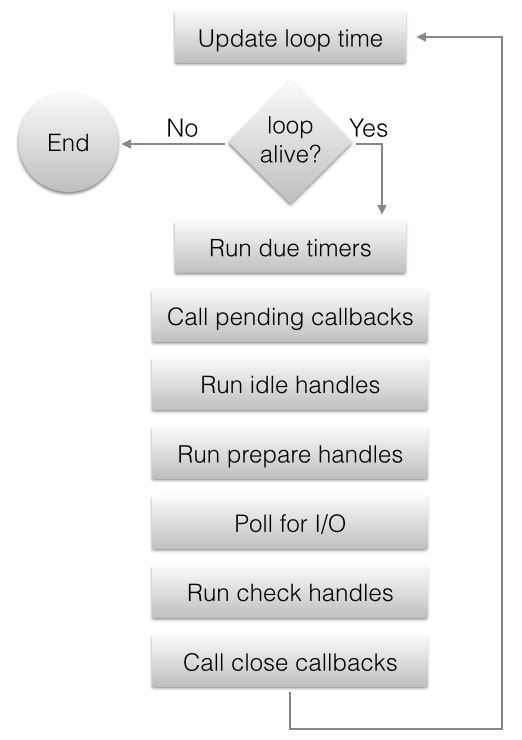
\includegraphics[width=7cm]{loop_iteration}
  \centering
  \caption[libuv event loop]{The stages each event loop iteration step through
  in libuv \cite{github2017libuv-loop_iteration}.}
  \label{fig:loop_iteration}
\end{figure}

Figure \ref{fig:loop_iteration} demonstrates the stages each event loop
iteration step through. A loop is considered to be alive if there are any
active handles or requests. For instance, if a TCP socket is closing its
connection the handle structure is freed from the heap and both the request and
handle are no longer active. If they were the last being active the loop dies.
The steps are described briefly: \cite{libuv-docs}

\begin{enumerate}
  \item The loop time is updated and stored for the entire iteration.
  \item If the loop is alive the iteration starts, otherwise it dies.
  \item All active timers who are scheduled to timeout have their callbacks
    called.
  \item Pending callbacks are called; they are I/O callbacks deferred from the previous
    iteration.
  \item Callbacks registered for idle handles are called. Idle handles are good
    for low priority activity.
  \item Callbacks that should be called right before polling for I/O can be
    registered with prepare handles, whose callbacks are called here.
  \item The time to poll for I/O is calculated here. It either blocks for 0
    seconds, the timeout for the closest timer or infinity. Depending on
    whether there are active idle handles or requests or if the loop is about
    to close, the time is 0. \label{item:poll_time_calculation}
  \item I/O is polled and the loop is blocked. All handles monitoring I/O will
    have their callbacks called.
  \item Callbacks that should be called right after polling for I/O can be
    registered with check handles, whose callbacks are called here.
  \item Handles being closed have their close callbacks called.
  \item If the loop was configured to only run once and no I/O callbacks were
    called after the poll, timers might be due since time could have elapsed
    during the poll. Those timers gets their callbacks called.
  \item Depending on the loop's configuration and if it is still alive, the
    loop exits or continue.
\end{enumerate}

The following example provided by Marathe \cite{uvbook} shows an idle handler
and its corresponding callback. As seen in Figure \ref{fig:loop_iteration} and
explained in step \ref{item:poll_time_calculation} idle handles and their
callbacks are called every iteration with 0 poll time.

\lstinputlisting[
  language=C,
  caption={libuv example with an idle handle \cite{uvbook}.},
  label={listing:idle_handle}
]{figures/libuv_idle_handle_example.c}

libuv includes a number of data types and functions which can be found in its
documentation \cite{libuv-docs}.

\section{Software maintainability}

Maintaining software has two distinct viewpoints: it could either be the act of
refactor and modify existing software to correct faults and improve existing
features, or it could point to the attribute of a software system that
expresses its ease of modification for the same purpose \cite{radatz1990ieee}.
Riaz et. al. \cite{riaz2009systematic} compiled a list of how other authors
that have studied maintainability in different settings defined the term
maintainability. The definitions could be \textit{"the ease with which a
software application or component can be modified to correct faults, improve
performance or other attributes, or adapt to a changed environment"} and
\textit{"how difficult it is to make small or incremental changes to an
existing software object without introducing errors in logic or design"}
\cite{riaz2009systematic}.

\todo{Continue here with stuff about metrics in general and the problem with
assessing them}

Previous research show that software process improvements is key for both large
and small successful companies. However, it requires a balance between formal
process and informal practice. Large companies tend to lean more towards the
formality of things and employees are given less space to be creative. On the
other hand, small companies tend to do the opposite: employees are given
freedom to explore solutions while formal processes are being put aside. Dybå
\cite{dybaa2003factors} suggests that "formal processes must be supplemented
with informal, inter-personal coordination about practice". It is also
important to note how failure is handled. Failure is essential for improving
learning and questioning the status quo inside both companies and software. If
failure is unacceptable, the organizational competance can decrease when facing
change in the environment. When a company is successful it will grow larger
with repeated success and there is no financial reason to change what already
works and generates revenue. However, eventually when the environment changes
there might be good reasons to dust off legacy systems and introduce some new
patches. The cost of doing so might depend on whether the system was initially
built with maintainability in mind. \cite{dybaa2003factors}

\subsection{Metrics}

In all engineering fields, measurement is important. Measuring software is a
way for an engineer to assess its quality and a large number of software
metrics have been derived during the years \cite{aggarwal2006empirical}.
Maintainability can be measured in many ways and Aggarwal et al.
\cite{aggarwal2006empirical} suggests that some metric results can be derived
from others. In the same way the area and diagonal can be derived from the
width and height of a table, some metrics may provide redundant information. It
is common, when selecting metrics to use in a study, that some metrics can be
superfluous in certain contexts or be substituted with similar metrics
\cite{benestad2006assessing} \cite{anda2007assessing}.

\todo{Some sort of leading text to the following subchapters}

\subsubsection{Halstead's metrics}

Metrics proposed by Halstead \cite{halstead1977elements} in 1977 are widely
used metrics that work both for object-oriented systems and non-object-oriented
systems \cite{al2005analysis} \cite{benestad2006assessing}. It consists of six
\textit{based} measures and ten \textit{derived} measures
\cite{al2005analysis}. Based measures are measures defined as an attribute and
the method used to measure it, and derived measures are defined as functions of
base measures \cite{al2005analysis}. The based measures are:

\begin{flalign*}
  &\text{Number of unique operators } n_1 &\\
  &\text{Number of unique operands } n_2 &\\
  &\text{Total number of operators } N_1 &\\
  &\text{Total number of operands } N_2 &\\
  &\text{Number of potential operators } n_1^* &\\
  &\text{Number of potential operands } n_2^* &
\end{flalign*}

These are self explanatory, except perhaps for the last two. $n_1^*$ and
$n_2^*$ are defined as the \textit{minimum} possible number for $n_1$ and
$n_2$. This depends on the programming language, but for C, where at least a
\lstinline{main()} function must be defined, $n_1^* = 2$ (the function name and
the parantheses symbols) and $n_2^* = 0$ (the number of required arguments to
\lstinline{main()}) \cite{menzies2002metrics}. To better understand the
measures, consider this sample program in C:

\begin{lstlisting}[language=C]
int main() {
  char s[12] = "Hello world!";
  printf(s);
  return 0;
}
\end{lstlisting}

The unique operators ($n_1$) are \lstinline{int}, \lstinline{main},
\lstinline{()}, \lstinline|{}|, \lstinline{char}, \lstinline{[]},
\lstinline{=}, \lstinline{"}, \lstinline{;}, \lstinline{printf} and
\lstinline{return}. The unique operands ($n_2$) are \lstinline{s},
\lstinline{12}, \lstinline{"Hello world!"} and \lstinline{0}. So $n_1 = 9$,
$n_2 = 4$, $N_1 = 14$, $N_2 = 5$.

The derived measures proposed by Halstead are:

\begin{flalign*}
  &\text{Program length } N = N_1 + N_2 &\\
  &\text{Vocabulary } n = n_1 + n_2 &\\
  &\text{Volume } V = N\log_2n &\\
  &\text{Potential volume } V^* = (2 + n_2^*)\log_2(2 + n_2^*) &\\
  &\text{Level } L = \frac{V^*}{V} &\\
  &\text{Difficulty } D = \frac{1}{L} &\\
  &\text{Level estimator \^{L}} = \frac{2n_2}{n_1N_2} &\\
  &\text{Intelligent content } I = \text{\^{L}} \times V &\\
  &\text{Programming effort } E = \frac{V}{L} = \frac{n_1N_2N\log_2n}{2n_2} &\\
  &\text{Programming time } T = \frac{E}{S} = \frac{n_1N_2N\log_2n}{2n_2S}
  \text{ ($S$ is usually set to 18 seconds \cite{hamer1982mh})} &
\end{flalign*}

Some critique on these metrics include a scattered counting strategy among its
users due to, among others, a vague definition of the difference between
operators and operands. Also, some of the derived measures are mathematically
equivalent which can cause confusion on their semantics. \cite{al2005analysis}

\subsubsection{Cyclomatic complexity}

Presented by McCabe in 1976 \cite{mccabe1976complexity}, the cyclomatic
complexity measure is a way to assess and measure the complexity of a code
block. It is defined as

$$
V(G) = e - n + 2p
$$

Where $e$ is the number of edges, $n$ the number of nodes and $p$ the number of
connected components. A software program can be presented as a \textit{control
graph} where each node represents a basic code block and each edge represents
branches taken by predicates such as if-statements. It is assumed that the
graph has only one entry point and one exit point and that each node can be
reached from the entry node, and that each node can reach the exit node. If the
exit node is connected to the entry node the graph is said to be
\textit{strongly connected}, and the cyclomatic complexity can be defined as
the number of linearly independent circuits. \cite{mccabe1976complexity}

\begin{figure}[h]
  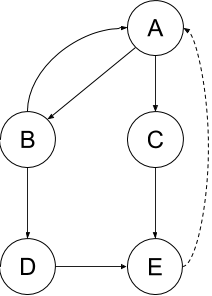
\includegraphics[width=4cm]{graph-1}
  \centering
  \caption{Control graph example}
  \label{fig:graph_1}
\end{figure}

In Figure \ref{fig:graph_1} a example is provided. Node $A$ is the entry point
and node $E$ is the exit point. Excluding the dotted edge connecting $E$ with
$A$, the graph has 6 edges, 5 nodes and represents one connected component;
i.e. $V(G) = 6 - 5 + 2 = 3$. Utilizing the connection between $E$ and $A$, the
same complexity value can be calculated by counting the number of linearly
independent circuits in the graph, i.e. the independent paths the program can
take. In this example the paths are $ABA$, $ABDEA$, $ACEA$, which corresponds
to the same result as $V(G)$.

Figure \ref{fig:graph_1} can be seen as a single program or control flow, e.g.
a function or class. Calculating complexity in a composition of functions or
classes, or the complexity of a function that calls other functions is
fortunately mathematically easy. The combined complexity of the graphs $G_1$
and $G_2$ is the sum of their respective complexities: $V(G_1 \cup G_2) =
V(G_1) + V(G_2)$. \cite{mccabe1976complexity}

The number of nodes and edges can be also be calculated by counting the number
of functions, predicates and collecting nodes in the program
\cite{mills1972mathematical}.  McCabe applies those relationships to the
cyclomatic complexity definition and reach the conclusion that the cyclomatic
complexity equals the number of predicates in the program plus one
\cite{mccabe1976complexity}. So complexity can be calculated as

$$
V(G) = \pi + 1
$$

where $\pi$ is the number of predicates in the program.

\subsubsection{Weighted Methods per Class (WMC)}

This metric relates to object oriented designs. Let $n$ be the number of
methods in a class and $c_i$ the complexity of method number $i$. Then the
metric is defined as:

$$
WMC = \sum_{i=1}^nc_i
$$

The more the methods and the higher their complexity value is, the higher the
maintainability effort is. \cite{chidamber1994metrics}

\subsubsection{Depth of Inheritance Tree (DIT)}

In object oriented programming, a class can inherit another class, i.e. be a
subclass of a superclass. This metric measures how many classes are inherited
all the way up to the root class. In programming languages like C++ where
classes can inherit multiple classes, the DIT is the longest distance to any
root class. \cite{chidamber1994metrics}

\subsubsection{Number of Children (NOC)}

This metric counts the number of classes that directly inherit a class, i.e.
its children. An advantageous viewpoint of this metric is that the more
children a class has, the greater the reuse of the class is. However, if a
class has a large amount of children it has a great effect on the design of the
system. \cite{chidamber1994metrics}

\subsubsection{Coupling Between Object Classes (CBO)}

An object is \textit{coupled} to another object of another class if it uses
methods or instance variables of that class. Coupling relates to the modularity
of a class, i.e. if a class has a high coupling value it is unlikely to be
reused or modified without having an effect on the coupled objects.
\cite{chidamber1994metrics}

\subsubsection{Response for a Class (RFC)}

When an object receives a message, e.g. a method is invoked, a potential set of
other methods can be called from that method. This metric measures the number
of those methods. A large RFC value can predict testing and debuging effort of
the class and its complexity. \cite{chidamber1994metrics}

\subsubsection{Lack of Cohesion in Methods (LCOM)}

Cohesion relates to the similarity of methods in a class. It is undesireable to
have a class design whose methods are not related to each other. This can be
measured by looking at the instance variables of the class and see how the
methods use them. If a class has $n$ methods, let $\{I_j\}$ be the set of
instance variables used by class $M_i$. Let $P$ be the number of instance
variable sets that has nothing in common, i.e. their intersection is
$\emptyset$. Let $Q$ be the opposite, i.e. the number of instance variable sets
whose intersection $\neq \emptyset$. Then $LCOM = |P| - |Q|$.
\cite{chidamber1994metrics}

\begin{gather*}
P = \{(I_i, I_j) | I_i \cap I_j = \emptyset\} \\
Q = \{(I_i, I_j) | I_i \cap I_j \neq \emptyset\} \\
LCOM = |P| - |Q| \text{, if $|P| > |Q|$, 0 otherwise} \\
\end{gather*}

\todo{More metrics like LOC, Maintainability Index and perhaps some machine
learning approaches. Also metrics that does not infer object oriented
languages.}

\subsection{Assessing maintainability}

Resulting numbers from a set of metrics applied on a software system can be
difficult to interpret; is the system maintainable or not? An alternative to
structural metrics can be subjective measures given by experts in the field.
Anda \cite{anda2007assessing} studied the correlation between structural
measures and expert assessments on four different software systems with
equivalent functionality and found that the both types of measures gave a
similar result. Interesting results have been found in a study by Sjøberg et.
al \cite{sjoberg2013quantifying} where certain bad design choices (or
\textit{code smells}) was hypothesized to lead to a greater maintenance effort.
However, the best predictor of maintenance effort turned out to be code size
and number of revisions of the software, i.e. small code bases are easier to
maintain. Benestad et. al. \cite{benestad2006assessing} applied several
measurement strategies in a similar context and cross examined the result. They
used class-level metrics, i.e. metrics applied on source code to make a
system-level assessment. An overall assessment strategy can be divided into
four categories; \textit{selection}, \textit{combination}, \textit{aggregation}
and \textit{interpretation}, which are explained further in the following
subchapters \cite{benestad2006assessing}.

How can the confidence behind an assessment be determined? Benestad et. al.
argue that if different assessment methods leads to the same result, one can be
confident in the result. They call it \textit{triangulation} and they use it in
their study. \cite{benestad2006assessing}

\subsubsection{Selection}

It is important to select metrics that best fit the systems under study. The
tools used to perform the metrics can play a big role in what metrics are used.
Also specific set of metrics, like the CK metrics \cite{chidamber1994metrics},
are often used. Using statistical analysis, an initial set of metrics can be
analysed to see if they discriminate between different designs. To avoid
applying superfluous, or \textit{unorthogonal}, metrics that does not influence
the resulting maintainability value to a certain degree, \textit{Principal
Component Analysis} can be used. \cite{benestad2006assessing}

\todo{Write about PCA!}

\subsubsection{Combination}

As ideal metrics only should measure one aspect of the design, and as
maintainability is affected by multiple aspects of the design, a combination of
several metrics are required to provide a fair image of a system's
maintainability value \cite{benestad2006assessing}.

Oman and Hagemeister \cite{oman1992metrics} proposes a quantitative approach
where multiple metrics can be combined into a unified value. Software
maintainability can be divided into three broad categories:

\begin{itemize}
\item The management practices being employed
\item Hardware and software environments involved in the target software system
\item The target software system
\end{itemize}

Oman and Hagemeister further derive the target software system into additional
categories:

\begin{itemize}
\item Maturity attributes
\item Source code
\item Supporting Documentation
\end{itemize}

Maturity attributes include metrics such as the \textit{age} of the software
since release, \textit{size} in terms of non-commented source statements and
\textit{reliability} which can be measured as the rate of failures per hour.
Source code include metrics on how the software is decomposed into algorithms
and how they are implemented, e.g. the number of modules and the cyclomatic
complexity averaged over all modules. It also includes metrics on the
information flow in the system, e.g. the number of global data types and
structures, the number of data structures whose type is converted and the
number of lines of code dedicated to I/O. Coding style metrics are also
included, e.g. the percentage of uncrowded statements (only one statement per
line), the number of blank lines and the number of commented lines are taken
into account. Supporting documentation are evaluated in a subjective manner.
Metrics include traceability to and from code implementation, verifiability of
the implementation and consistency of the writing style and comprehensibility
of the document. \cite{oman1992metrics}

To assess these metrics, Oman and Hagemeister introduces a formula:

\begin{align*}
\prod_{i=1}^m{W_D_i(\frac{\sum_{j=1}^n{W_A_jM_A_j}}{n})_i}
\end{align*}

where $W_D_i$ is the weight of influence of software maintainability category
$D_i$, e.g.  source code control structure. $W_A_j$ is the weight of influence
of maintainability attribute $A_j$, e.g. software age. $M_A_j$ is the measure
of maintainability attribute $A_j$. The values should be structured so that
they range from 0 to 1, thereby showing a percentage of their correctness.
Worth noting is that not all attributes have to be measured, only those of
significant value. \cite{oman1992metrics}

Coleman et. al. \cite{coleman1994using} proposes a polynomial model that
includes four metrics. By using regression analysis \todo{Elaborate further on
regression analysis?} on historical data they were able to adjust the values in
the polynomial to make a good maintainability prediction. The formula is
expressed as:

\begin{align*}
\text{Maintainability} = 171 \\
  - 5.2 \times \ln(\textit{aveVol}) \\
  - 0.23 \times \textit{ave$V(g')$} \\
  - 16.2 \times \ln(\textit{aveLOC}) \\
  + 50 \times \sin(\sqrt{2.46 \times \textit{perCM}})
\end{align*}

Where \textit{aveVol} is Halstead's volume metric averaged over all source code
modules, \textit{ave$V(g')$} is the extended cyclomatic complexity \todo{how
does that differ from "normal" $V(g)$?}, \textit{aveLOC} is the average number
of lines of code and \textit{perCM} is the percentage of comments across all
modules. \cite{coleman1994using}

\subsubsection{Aggregation}

Aggregating results from software metrics is a statistical task. Metric values
can be distributed in various ways, making fair interpretation hard. The most
popular approach is taking the mean value of a specific metric, across all
modules. A problem with this approach is, say one module has a very high
complexity value while another has a very low, the resulting mean value will be
a compensation right in between. A better approach in that case can be to
measure the standard deviation of each metric that will give a hint on how
evenly a certain metric is spread out across the modules, which leads to a
notion of how balanced the design is. \cite{benestad2006assessing}

\begin{ctable}
  {Aggregation example found in an article by Anda \cite{anda2007assessing}.
  The values can be read on the format $<mean>/<standard deviation>$.}
  {l r r r r}
  \label{tab:aggregation_example}
  \multicolumn{2}{r}{\textbf{A}} &  \textbf{B} &  \textbf{C} &  \textbf{D} \\
  \hline
  \textbf{WMC} &  6.9/11.2 &    7.8/10.3 &    11.4/12.5 &   4.9/4.5 \\
  \hline
  \textbf{NOC} &  0.46/2.75 &   0.59/2.37 &   0/0 &         0.76/3.81 \\
  \hline
  \textbf{DIT} &  0.46/0.5 &    0.75/0.81 &   0/0 &         0.83/0.54 \\
  \hline
\end{ctable}

Table \ref{tab:aggregation_example} shows the result of some metrics applied on
four systems A-D, each developed by different software teams but following the
same specification. System C uses no inheritance functionality, hence the zero
value for number of children (NOC) and depth of inheritance tree (DIT). All
systems have a relatively high standard deviation, meaning the measures differ
between classes and are quite unbalanced. \cite{anda2007assessing}

\subsubsection{Interpretation}

Interpretation can be used as a final step in the maintainability assessment
procedure in order to find a relationship between the internal, structural
measures and the external quality attributes of the system. A level of
uncertainty will always be present in interpretation and depending on the
intended use of the measurement results, the appropiate uncertainty level
changes. By simply looking at the resulting values from a combined or
aggregated measurement, a maintainability assessment can be made. Low values
can indicate bad maintainability and vice versa (or reverse). This is called
\textit{relative interpretation} and, though being simple, has its drawbacks.
In object oriented languages, a deep class inheritance tree can be interpeted
to be complex and result in bad maintainability. But in the opposite case, a
flat class hierarchy means object oriented features are not used, which also
can be interpreted as bad maintainability. Another interpretation strategy is
the use of \textit{threshold values} that are discrete intervals in the
possible value space of the structural measures. Thresholds can be labeled
\textit{Good}, \textit{Acceptable}, \textit{Suspicious} and
\textit{Unacceptable}. \textit{Sensitivity analysis} may be needed when
threshold values are used. Depending on the thresholds used the outcome can
differ and therefore it can be valuable to try different threshold values. If
the thresholds produce very sensitive outcomes the confidence of the
maintainability result is low. \cite{benestad2006assessing}

\subsection{Measuring maintainability in C++}

Some metrics might not be suitable for object-oriented (OO) languages and C++
in particular. Wilde and Huitt \cite{wilde1991maintenance} studies some of the
main difficulties regarding maintenance as in "post deployment support" of
OO-languages. These languages introduces the concepts of \textit{object class
inheritance hierarchy} and \textit{polymorphism} which in some sense helps give
programmers a better understanding of their programs, but the maintenance
burden will unlikely disappear completely. One issue with analyzing OO source
code is \textit{dynamic binding}. An object variable might not necessarily
refer to its declared class type, but it can also refer to any of its
descendants in the class hierarchy. This makes static analysis complicated,
e.g. it is not always known what implementation of a method will be used when
the method is called on an object.

Rajaraman and Lyu \cite{rajaraman1992reliability} have also studied the
shortcomings on some traditional maintainability metrics on OO-languages. For
instance, they look on the metric \textit{statement count} which can predict a
software's complexity. It is built on the assumption that "the more detail that
an entity possesses, the more difficult it is to understand"
\cite{rajaraman1992reliability}. The metric simply counts the number of
statements in a program or module. They criticize the metric for not taking the
program's context into account and that it is not easy to determine what
exactly a statement is. They also criticize McCabe's
\cite{mccabe1976complexity} \textit{cyclomatic complexity measure} that
calculates a program's complexity by taking the number of edges in a program
flow graph, the number of nodes and the number of connected components into
account (nodes are abstractions of sequential blocks of code and edges are
conditional branches in the program). The critique involves, as stated earlier
regarding statement count, that the metric ignores the context in the program
and has no support to take the complexity of each statement into account.

Rajaraman and Lyu \cite{rajaraman1992reliability} defines four measures of
\textit{coupling} in their paper. They define the term coupling as "[...] a
measure of association, whether by inheritance or otherwise, between classes in
a software product". Abstracting the program to a directed multigraph, each
node represents a class and each edge represents a reference from one node to
another through variable references and method calls. Two of the proposed
measures, \textit{Class Coupling} and \textit{Average Method Coupling} resulted
in highest correlation (though not statistically significant) with perceived
maintainability when tested on a number of C++ programs. Class Coupling for a
class $C$ is defined as the sum of each outgoing edge from $C$; i.e. the sum of
all global variable references, all global function uses, all calls to other
class methods and all local references to other class instances. Average Method
Coupling is a ratio number between a class $C$'s Class Coupling and its total
number of methods, i.e. $AMC = CC / n$ where $n$ is the total number of methods
declared in $C$.

\section{Performance testing}

Performance testing is the process of measuring and evaluating certain
performance related benchmarks in a system; usually by putting the system under
I/O load such as simulated network traffic \cite{jiang2015survey}. Software
systems contains resources such as the CPU, processes, threads and I/O that all
have limited capacities, which mean they potentially can deny each others
execution when several users require the same resource. Analysing a system's
performance require quantification of such effects \cite{woodside2007future}.
The goal of the tests could be to compare an existing system with a new
proposed system to see which one performs better \cite{avritzer1996deriving} or
to, in an early phase of the development of a system, identify future
performance problems upon deliverance \cite{weyuker2000experience}. Contrary to
functional software testing where the values of the test inputs determines the
test outcome, performance testing emphasizes the \textit{workloads} and
\textit{frequencies} of the inputs \cite{weyuker2000experience}. Jiang and
Hassan discusses performance testing along with two other similar testing
techniques: \textit{load testing} and \textit{stress testing}
\cite{jiang2015survey}. Load testing is defined as the process of assessing a
system's behavior under load to find both functional and non-functional related
issues. Stress testing is about putting the system under extreme load
conditions to verify robustness.  Performance testing differ from the other two
when it comes to verification of benchmarks. A performance test can for
instance happen when a module has been reengineered and the performance must be
verified to at least be as good as the previous version of the module
\cite{jiang2015survey}.

Usually, performance tests objectives relates to I/O throughput and response
time. Weyuker and Vokolos conducted performance tests on a telecommunication
gateway by developing simulated telephone callers \cite{weyuker2000experience}.
These callers performed calls and transactions on the systems that were
measured to analyse performance. Performance metrics used by the popular
performance testing tool \textit{JMeter}\footnote{See
\url{jmeter.apache.org}.}, which is often used to test web applications and
services, include \cite{mendelawy2016kpis}:

\begin{description}
  \item[Number of Users:] Measuring the number of active users can be done by
    creating \textit{virtual users} in a testing program. This metric is at
    most interesting when analysed together with Hits per Second.
  \item[Hits per Second:] This is a measure on how many requests are generated
    by each user. The correlation between Number of Users and Hits per Second
    provides a valuable hint on the performance of the server.
  \item[Errors per Second:] A high error rate when the user amount increases
    indicates a performance issue.
  \item[Response Time:] The time it takes from a request to its response is,
    especially when multiple requests are fired concurrently, a good indication
    on the performance of the system.
  \item[Throughput:] This measures the average bandwidth usage generated by the
    tests.
\end{description}

To conduct a performance test, not only are the metrics necessary, but a
representative workload is needed as well \cite{weyuker2000experience}.
Methods to design workloads often requires historical data on what load the
system undergoes in typical usage. But as performance testing usually is
performed on novel systems, historical data is a rare commodity
\cite{barber2004creating}. Alternative approaches can be to retrieve usage data
from a beta version of the system, have interviews with domain experts or
analyse usage data from competitors \cite{jiang2015survey}. Barber synthesizes
common approaches found in the industry and provides a, somewhat agile,
framework to support design of a workload model where historical data is
incomplete or unavailable \cite{barber2004creating}:

\begin{enumerate}
  \item Identify existing historical data, preferably found in log files from
    production instances of the system.
  \item If log files are unavailable, try to extract information from
    stakeholders such as salesmen (they might know of the most anticipated
    activities that can be used in the workload design) and users (they might
    know what activites they probably will do).
  \item Look for performance related activites in design and requirements
    documents.
  \item Whenever a new beta version of the system is available, retrieve
    workload data from it.
  \item Look for workload data in competitors' statistics if available.
  \item Conduct in-house experiments.
  \item If no data is available, use personal experience as a substitute to
    design an appropiate model.
  \item Create visual representations of the model for peer review.
  \item Create three different workload models based on:
    \begin{enumerate}
      \item Anticipated or expected usage.
      \item Best case usage.
      \item Worst case usage.
    \end{enumerate}
\end{enumerate}

Jiang and Hassan suggests workload models can either reflect the system's
performance requirements (so called \textit{aggregate-workload based load
design}) or the system's expected usage (\textit{use-case based load design}).
An example of a performance requirement can be that CPU usage should not exceed
90 \% when 10,000 transactions are concurrently handled. Expected usage can be,
for a web shop application, that users typically spend 40 \% of their time
browsing and 60 \% in the checkout. In the aggregate-workload approach loads
are characterized as the \textit{workload intensity}, i.e. the rate in which
the requests fire, and the \textit{workload mix}, which describes the different
kinds of requests in the workload, e.g. 20 \% of the requests come from
resource $A$ and 80 \% from resource $B$. For cases where historical data or an
operational profile is available, a workload model can be designed as
\textit{steady load} or \textit{step-wise load}. In a steady load, only one
intensity and mix configuration is used, normally to represent expected usage
of the system. However, a better representation of a realistic workload would
be one where the workload varies with time. A step-wise load include multiple
levels of workload intensity (but keeps the workload mix) to mimic certain
usage levels across a time period. The main disadvantage with the
aggretage-workload approach is that loads can be unrealistic or hard to design.
The use-case approach tries to solve this by introducing states and stochastic
aspects into the design. One can for instance design loads using \textit{use-case
diagrams}, \textit{Markov chains} and \textit{Probabilistic Timed Automata} to
create usage driven designs that resemble real-world workloads. \cite{jiang2015survey}

\todo{How to execute performance test?}

\section{Software development methodology}

There exists a numerous amount of ways to develop software. In plan-based
methodologies, including the \textit{waterfall model}, the way of working is
highly inspired by traditional engineering such as manufacturing and
construction. Given a set of phases in the development, each phase must be done
before the next phase starts. These phases include \textit{requirement
definition}, \textit{design}, \textit{implementation}, \textit{testing} and
\textit{release} \cite{crookshanks2014practical}. On the other end of the
spectra lies the \textit{agile} methodologies. Initially developed as a
response to the frustration of the static, slow-going process of the well-used
waterfall model, it is based on the understanding that software requirements
are highly dynamic and most certainly change over time
\cite{moniruzzaman2013comparative}.

Vijayasarathy and Butler \cite{vijayasarathy2016choice} found in an online
survey they conducted in 2016 that around a third of all software projects were
using the waterfall model as main software methodology. Following were the
agile methodologies \textit{Agile Unified Process} and \textit{Scrum}. They
also found that multiple methodologies were often used in the same project.
For instance the agile method \textit{Joint Application Development} was used
in one project to identify requirements, while the waterfall model was used in
the remainder of the project.

\subsection{Scrum}

Scrum is an agile framework utilized by small teams to develop simple and
complex products. Scrum is not only used to do software development, it can be
applied to any development - even a book \cite{sims2012scrum}. In Scrum there
are three main components: \textit{roles}, \textit{artifacts} and \textit{the
sprint cycle}. Roles are taken by people in the team, artifacts are tools used
by the team and the fundamental pulse of the project is the sprint cycle. Three
distinct roles are recognized: \textit{product owner}, \textit{Scrum master}
and \textit{team member}. The product owner is the team's representation of the
\textit{stakeholders} of the product (mainly the business related
stakeholders). He is responsible for making the team always do most valuable
work, he holds the vision of the product, he owns the \textit{product backlog}
and creates acceptance criteria for the backlog items. The scrum master is the
team's coach guiding them to become a high-performing, self-organizing team. He
helps the team apply and shape the agile practices to the team's advantage. A
team member is responsible for completing \textit{user stories}, create
\textit{estimates} and decides what tools to use in the upcoming
\textit{sprint}. \cite{sims2012scrum}

The artifacts recognized by Scrum are called \textit{product backlog},
\textit{sprint backlog}, \textit{burn down charts} and \textit{task board}. The
product backlog consists of a list deliverables that can be anything of value
for the product, e.g. features and documentation changes. Items in the list are
also called \textit{user stories} and they are ordered by priority. They
include information such as who the story is for, what needs to be built, how
much work is needed to implement it and what the acceptance criteria is. Prior
to a \textit{sprint} user stories are derived into practical \textit{tasks}
usually performed by a single team member. The sprint backlog is populated by
these tasks and they are expected to be finished within the time limit of the
sprint. To monitor the status of the sprint or the entire project, the burn
down chart is used. It is a diagram showing how much work is left to be done.
The Y-axis shows the amount of tasks and the X-axis the time. As time progress
the amount of tasks are hopefully decreasing. The task board is used to help
the team inspect their current situation. It usually consists of three columns:
\textit{To do}, \textit{Doing} and \textit{Done}. Each column consists of tasks
(or symbols of tasks) in the current sprint, and gives the team a visual on
what tasks are yet to be done. \cite{sims2012scrum}

A Scrum project is split into a series of sprints. They are time limited
smaller versions of the entire project where a pre-defined amount of tasks are
to be completed within the sprint. When a sprint is finished a potentially
working product is demonstrated. The benefit of short-lived sprints is that the
team receives frequent feedback on their work, giving them a better presumption
to improve future sprints. From a business perspective, the sprint method
provides greater freedom to decide if a product should be shipped or further
developed. A sprint consists of a number of meetings: \textit{sprint planning},
\textit{daily Scrum}, \textit{story time}, \textit{sprint review} and
\textit{retrospective}. A sprint always starts with a sprint planning. It is a
meeting where the product owner and the team decides which user stories will be
a part of the sprint backlog in the upcoming sprint. This is also where the
team derive the user stories into tasks. Every day the team also has brief
daily Scrum meetings. Each team member shares what tasks they completed since
the previous meeting, what tasks they expect to complete before the next and
what difficulties they are currently facing. Every week, during story time, the
product backlog is again reviewed by the team and the product owner. This time
each user story is evaluated to refine its acceptance criteria. If there are
large stories in the backlog they are also split into smaller stories to make
them easier to understand and easier to complete within a sprint. The sprint
review marks the public end of the sprint. Here the completed user stories are
demonstrated to the stakeholders and feedback is received. After this meeting
the team has a retrospective meeting where they discuss what strategy changes
can be made to improve the next sprint. \cite{sims2012scrum}

